\chapter{Estrutura do Projeto}
\label{sec:estrutura}

  Esse capítulo tem o objetivo de expor o conceito que projetamos para nosso
  sistema. Existe uma certa complexidade em entender como os diversos
  componentes dele se relacionam - principalmente devido ao fato deles usarem
  técnicas como geração de código automatizada e análise reflexiva de código. A
  ideia por trás dessas técnicas também serão explicadas nesse capítulo.
  
  A seção \ref{sec:estrutura:geral} buscará deixar
  claro o contexto em que o projeto funciona e como as responsabilidades
  são distribuídas para atingir a solução modelada. As seções
  \ref{sec:estrutura:opa} e \ref{sec:estrutura:opwig} detalham as duas
  principais partes do projeto, e a seção \ref{sec:estrutura:integration}, por
  fim, explica como tudo isso funciona em conjunto para atender às necessidades
  do usuário.

  \section{Visão Geral}
  \label{sec:estrutura:geral}
  
    Um usuário do nosso sistema estará tipicamente desenvolvendo uma aplicação
    em uma linguagem compilada (mais especificamente, \CXX{}) que de alguma
    forma precisa interagir com uma linguagem de \script{}. Essa interação pode
    ser estabelecida diretamente entre elas se a máquina virtual da linguagem de
    \script{} em questão tiver sido programada na linguagem compilada usada,
    pois isso dará acesso:
    
    \begin{itemize}
      \item[(A)]
        À API própria da máquina virtual que permite que ela seja manipulada
        através de sua linguagem nativa.
      \item[(B)]
        Ao protocolo com o qual \script{s} podem pedir à máquina virtual acesso
        a recursos programados na linguagem nativa dela.
    \end{itemize}

    Esses dois elementos estabelecem duas vias de interação entre as linguagens
    envolvidas. Através de (A) a linguagem compilada pode acessar e manipular
    elementos da linguagem de \script{}, enquanto que usando (B) o contrário é
    possível. O propósito do sistema que desenvolvemos é abstrair e automatizar
    o uso dessas duas vias para minimizar o esforço que o usuário necessita para
    desenvolver a interação desejada na sua aplicação.

    \begin{figure}[ht]
      \centering
      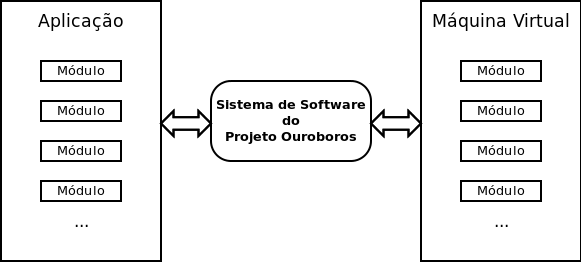
\includegraphics[width=.8\textwidth]{overview-simple.png}
      \caption{Esquematização bem simplificada do sistema.}
      \label{fig:overview-simple}
    \end{figure}

    Vamos dizer que tanto a aplicação quantos os \script{s} estão divididos
    em \textbf{módulos}. Eles serão os objetos das interações tanto do tipo (A)
    quanto do tipo (B), representando o conjunto de elementos provenientes de
    uma ou de outra linguagem que podem ser acessados e manipulados. Por
    exemplo, se a aplicação do usuário for um jogo de ação no qual o jogador
    enfrenta inimigos virtuais, ele poderia usar \script{s} para implementar a
    inteligência artifical desse inimigos, para que fosse fácil ajustá-las sem
    ter que re-compilar o jogo. Desse modo, cada um desses \script{s} seria um
    módulo que a aplicação precisaria carregar e usar durante sua execução.
    Eles, por sua vez, precisariam interagir com módulos da aplicação para que
    as inteligências artificiais conseguissem manipular seus personagens dentro
    do mundo virtual do jogo.

    Dessa forma, uma primeira ilustração bem simplificada da estrutura geral do
    nosso sistema é a representada na Figura \ref{fig:overview-simple}. Existem
    vários fatores que estão sendo omitidos nesse esquema, principalmente
    envolvendo a interação do tipo (B). Além disso, ainda não foi dito
    explicitamente o que significam essas interações. Esses e outros detalhes
    serão aprofundados nas seções a seguir.
    
    % TODO: Definir melhor os atos de "exportar" e "importar" entre as
    %       linguagens

  \section{Biblioteca de abstração de APIs de linguagens de \emph{script}.}
  \label{sec:estrutura:opa}
  
  Uma máquina virtual de uma linguagem de \script{} é implementada em uma outra
  linguagem, que chamamos de sua linguagem nativa. Enquanto nosso sistema trabalha
  com as linguagens nativas \C{} ou \CXX{}, podem existir implementações da máquina
  virtual para diversas linguagens. É comum a implementação de uma máquina virtual
  disponibilizar uma API para sua linguagem nativa, provendo funções, constantes
  e outros elementos para que a linguagem nativa consiga acessar e manipular a
  máquina virtual e seu conteúdo. Isso na prática que representa a interação do
  tipo (A).

  Infelizmente, para um usuário comum que está desenvolvendo um programa em
  linguagem nativa, usar a API de uma máquina virtual é normalmente uma tarefa
  difícil e trabalhosa pela complexidade da API e do tempo para aprender a 
  usá-la. Foi para resolver esse problema que desenvolvemos a biblioteca de 
  abstração de APIs de linguagens de \script{}, também conhecida como 
  \textit{libouroboros} ou simplesmente como \emph{Ouroboros Project API} (OPA).
  
  A libouroboros é a parte do nosso projeto que provê a interação do tipo (A),
  como explicada acima. Ela consiste em um conjunto de classes e funções em 
  \CXX{} que generalizam o meio com o qual se realiza diversas operações com 
  a API da linguagem de \script{}, como:
  \begin{itemize}
    \item carregar um \script{};
    \item executar uma função na máquina virtual;
    \item pegar/configurar um objeto/atributo/valor na máquina virtual;
    \item converter valores entre linguagem nativa e a máquina virtual;
  \end{itemize}
  Parte desse conjunto de classes define uma interface que deve ser implementada para
  cada linguagem de \script{}, possibilitando que o sistema reconheça tal linguagem e 
  realize as operações descritas. Essa implementação usa diretamente a API da linguagem
  para satisfazer nossa interface. Em contrapartida, tal implementação é usada pelo 
  resto do sistema. Desse jeito, o usuário final do OPA não precisa usar esses 
  componentes, nem se preocupar com a API da linguagem de \script{}, a não ser que
  ele vá adicionar o suporte a ela no sistema.

  % TODO: Diagrama ilustrando relação da OPA com as APIs específicas de cada
  %       linguagem de script
  
  Por padrão, o projeto já tem a implementação de \textit{Lua} e \textit{Python}.
  
  %TODO: subsection: conversão de valores (entre linguagem nativa e máquina virtual)
  %TODO: subsection: virtualobj (possiveis subsubsection pra falar do encapsulamento do vdata, etc)
  %TODO: subsection: importação de um módulo de script para a linguagem nativa
  
  
  \section{Gerador de \emph{wrappers} e interfaces.}
  \label{sec:estrutura:opwig}

  %TODO: Explicar mais sobre a ideia geral da relação do tipo (B)

  Linguagens de \script{} possuem um mecanismo próprio para importar os módulos
  necessários à sua execução. Esses módulos podem ser definidos tanto em outros
  arquivos na mesma linguagem, quanto na linguagem nativa da máquina virtual.
  Nesse último caso, temos a relação do tipo (B). Ela exige que a linguagem
  nativa disponibilize certos dados seguindo um protocolo adequado. Infelizmente
  tal protocolo não só difere para cada linguagem de \script{} como também
  involve um trabalho repetitivo e maçante para ser utilizado. 
  
  Por isso, parte do nosso sistema é composta por um gerador automatizado de código fonte.
  Ele é responsável por criar o código necessário ao devido funcionamento dos módulos 
  feitos na linguagem nativa. Além disso, ele processa código que o usuário fornecer na
  linguagem nativa para saber o conteúdo que deve aparecer no módulo exportado.
  Esse conteúdo é inserido no módulo através de \emph{wrappers}. Chamamos esse componente
  do sistema de \emph{Ouroboros Project Wrapper and Interface Generator} (OPWIG).
  
  %TODO: subsection: parser
  %TODO: subsection: code generator
  %TODO: subsection: wrapper explanation 
  
  \section{Integrando e entregando tudo para o usuário.}
  \label{sec:estrutura:integration}
  TODO
